\documentclass{article}

\usepackage[final]{style}
\usepackage[utf8]{inputenc} % allow utf-8 input
\usepackage[T1]{fontenc}    % use 8-bit T1 fonts
\usepackage{hyperref}       % hyperlinks
\usepackage{url}            % simple URL typesetting
\usepackage{booktabs}       % professional-quality tables
\usepackage{amsfonts}       % blackboard math symbols
\usepackage{nicefrac}       % compact symbols for 1/2, etc.
\usepackage{microtype}      % microtypography
\usepackage{verbatim}
\usepackage{graphicx}       % for figures
\usepackage{float}

\title{Lecture \#8: Model-Based RL and Policy Learning}

\author{
  Nick, Nan and Halder 
}

\begin{document}

\maketitle


\section{Introduction}

\noindent\textbf{Problems for backpropagating directly into policy} 

\begin{figure}[H]
    \centering
        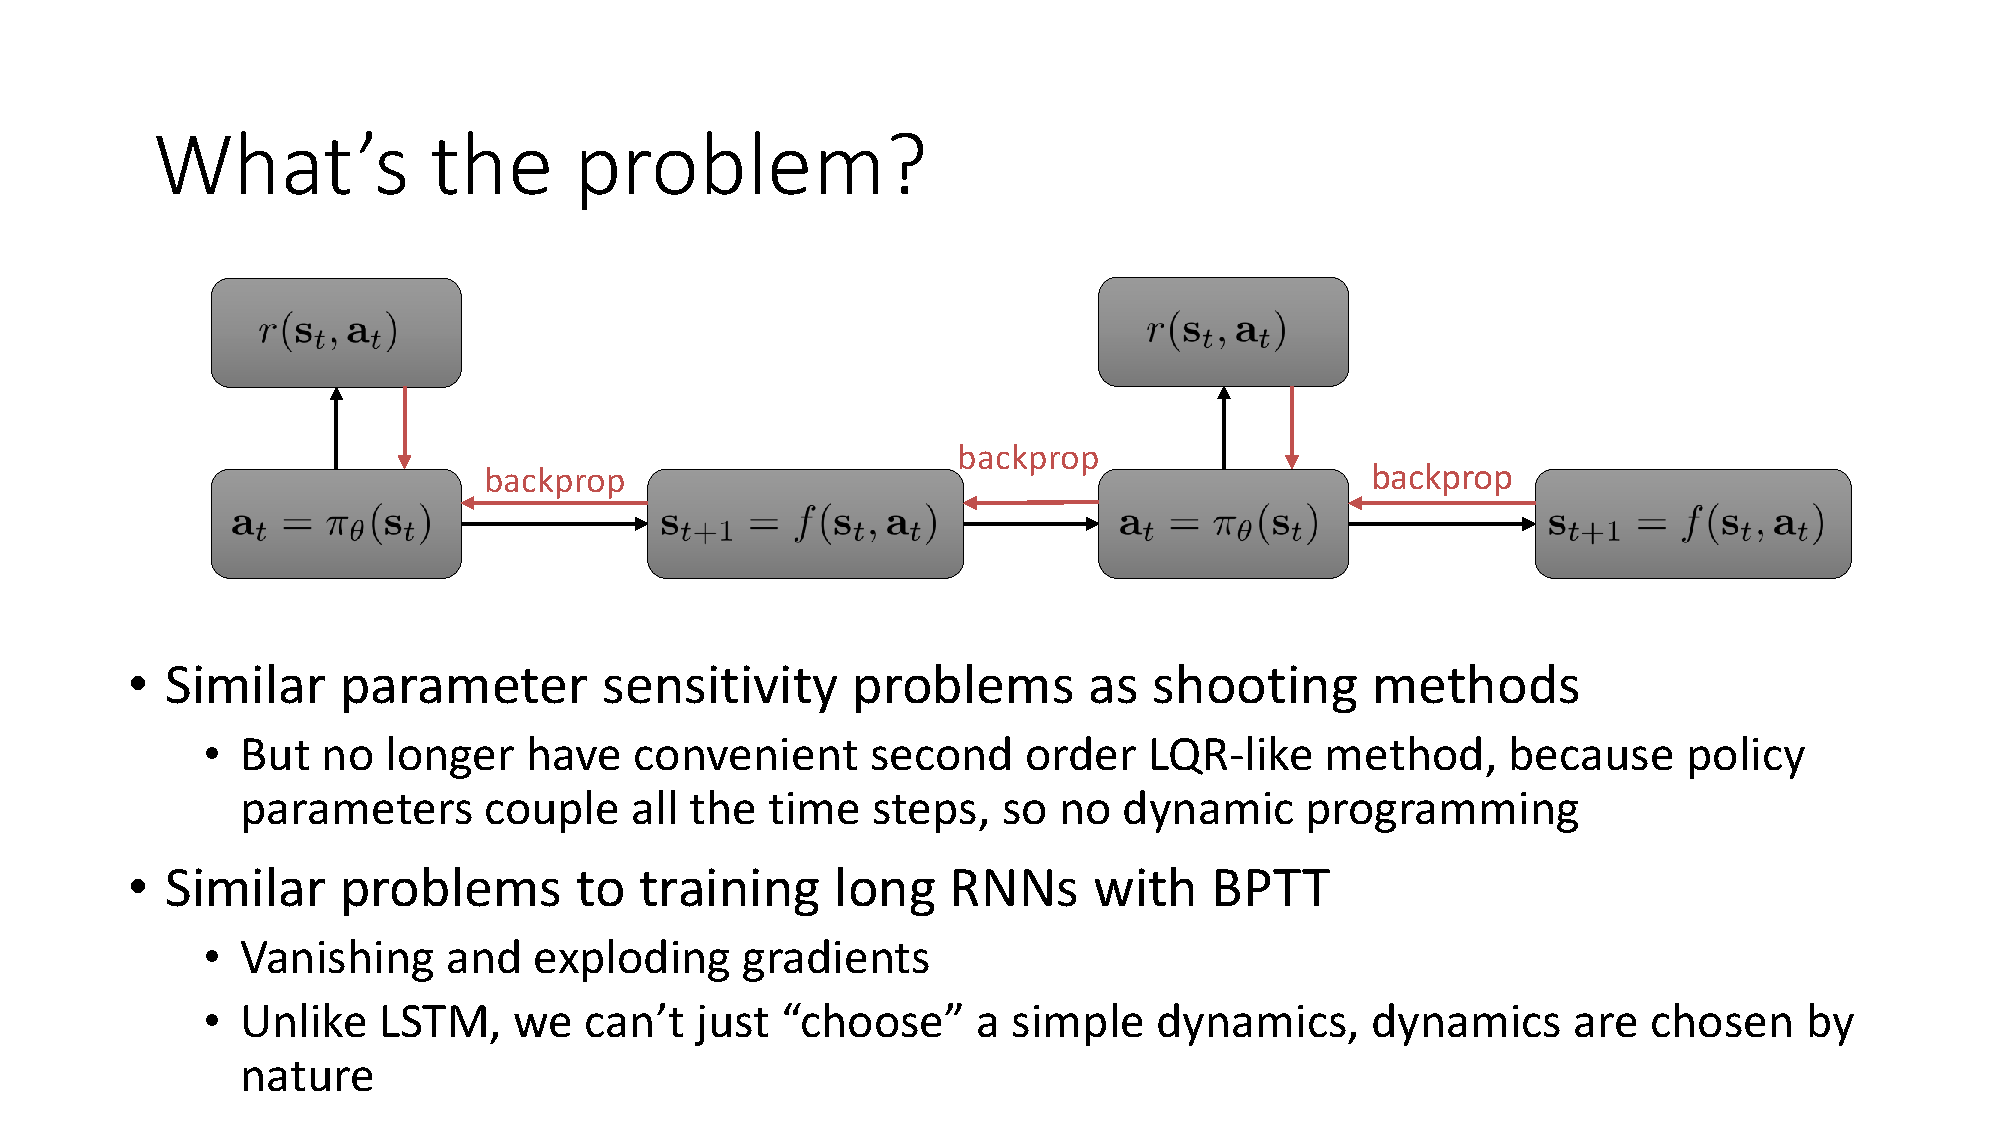
\includegraphics[width=0.8\linewidth]{img/whats_the_problem.png}
\end{figure}

\begin{figure}[H]
    \centering
        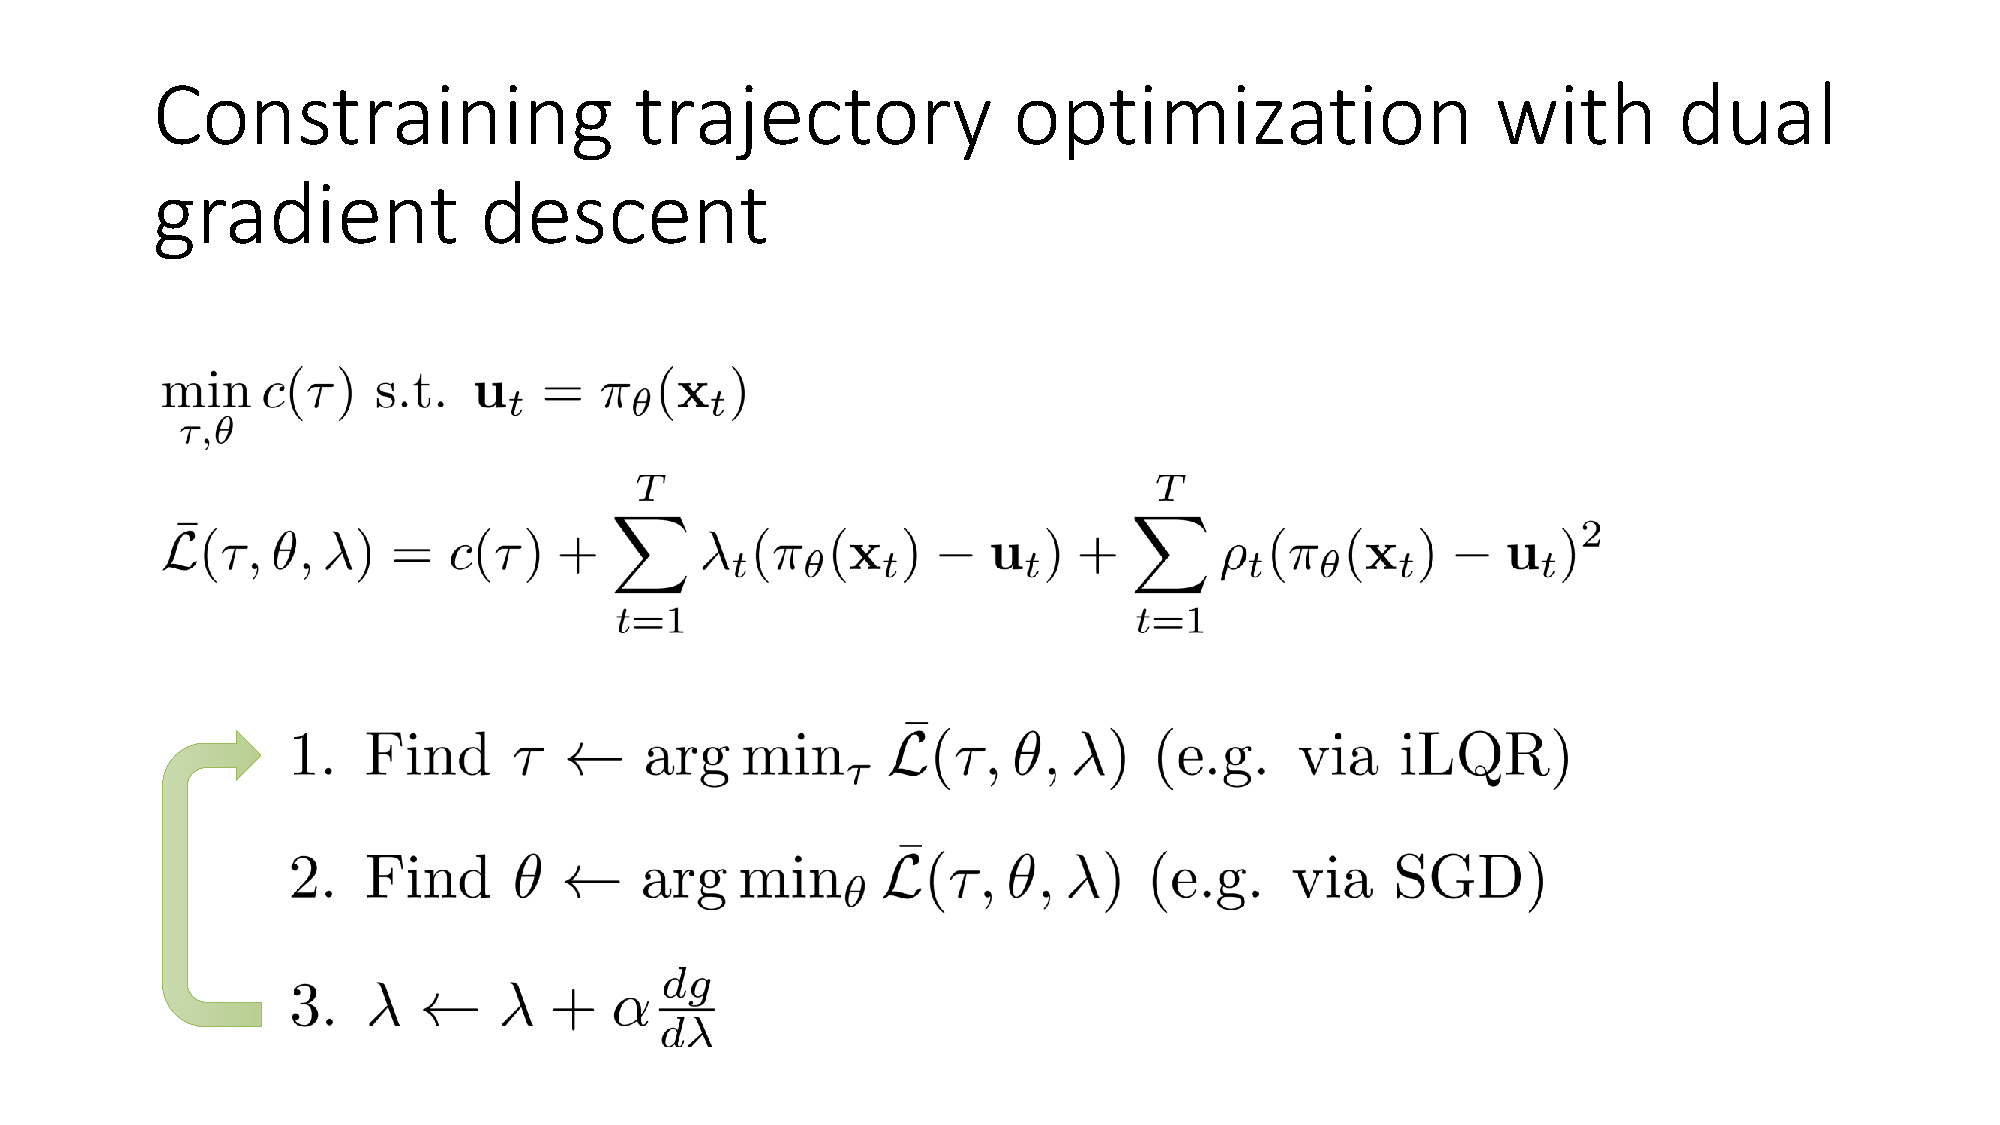
\includegraphics[width=0.8\linewidth]{img/dual_gradient.png}
\end{figure}

\begin{figure}[H]
    \centering
        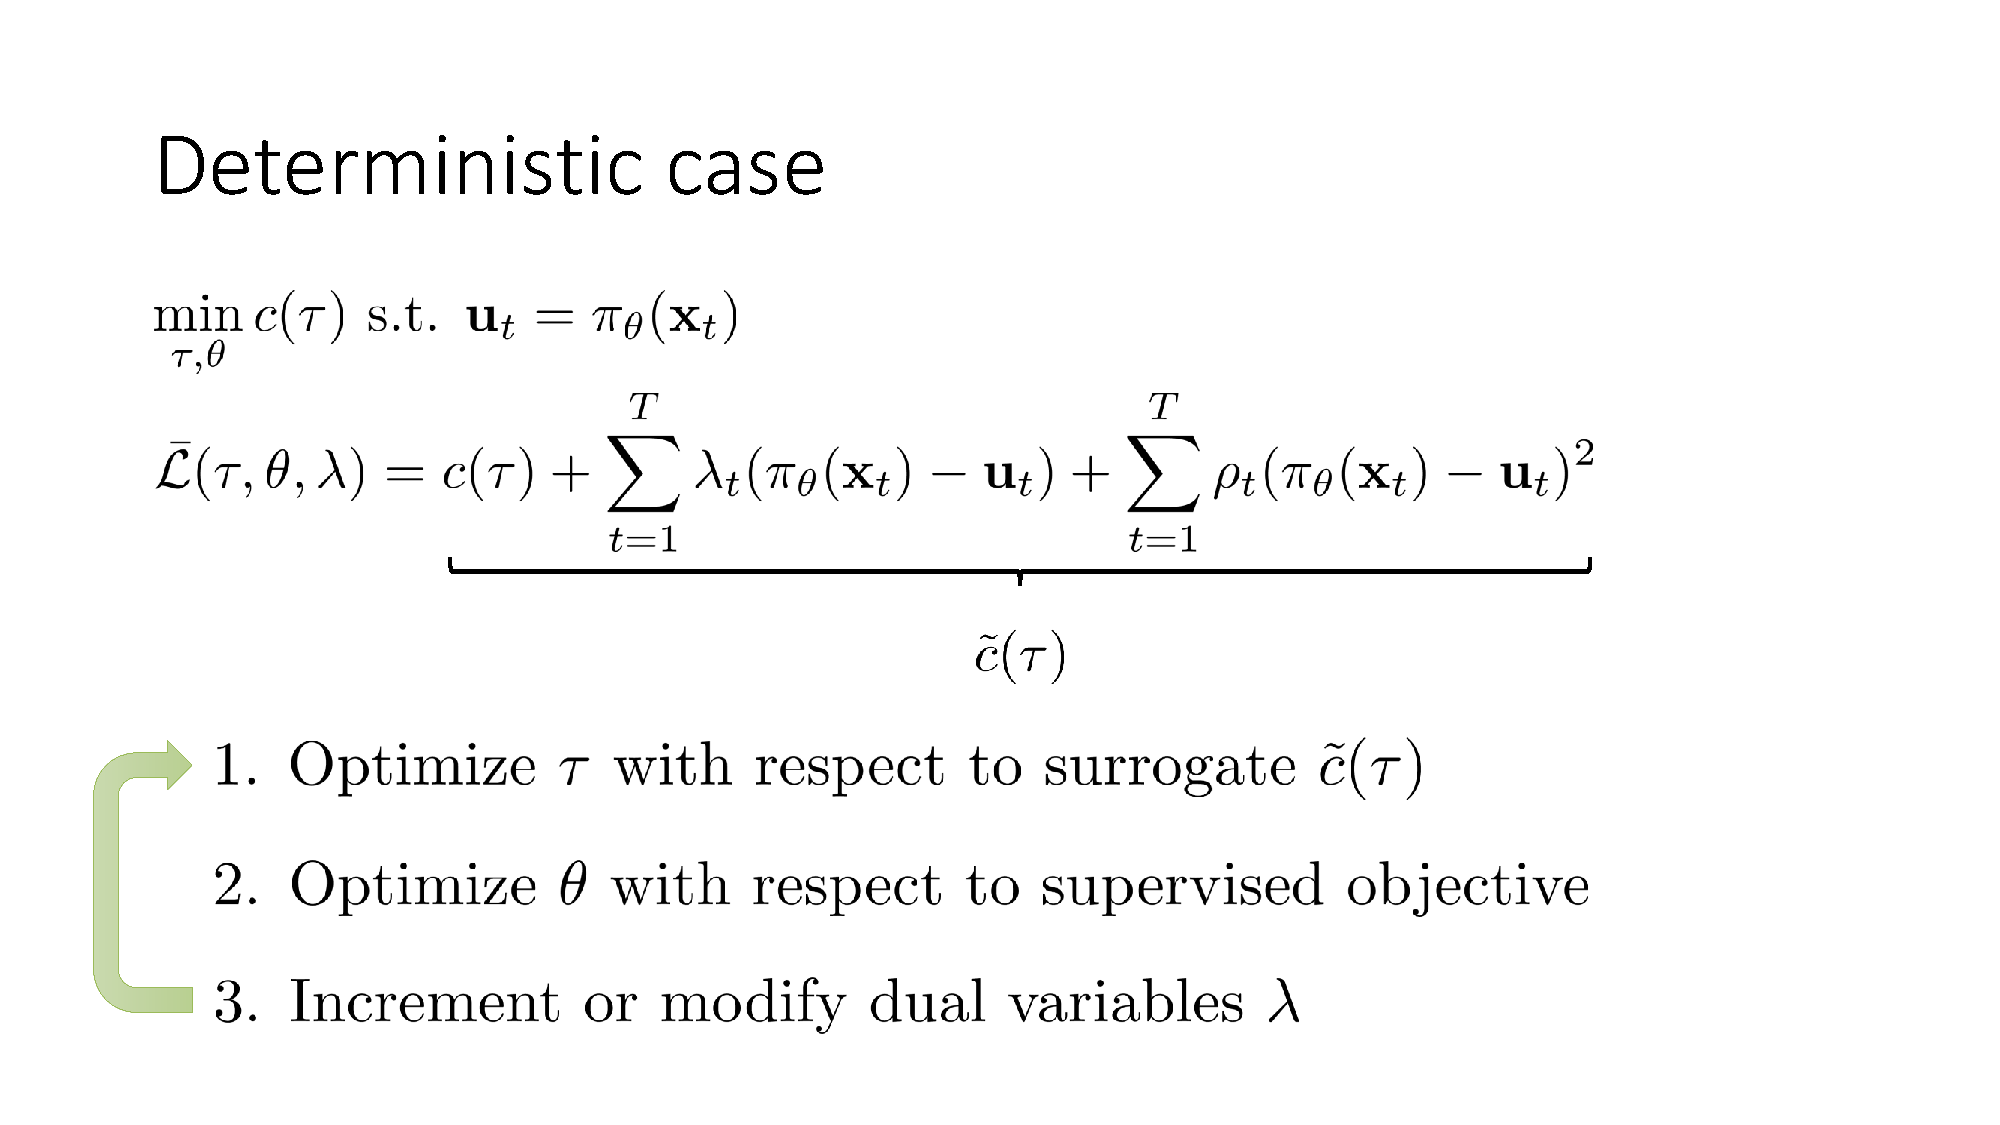
\includegraphics[width=0.8\linewidth]{img/determinstic_case.png}
\end{figure}

\noindent\textbf{GPS} 

\begin{figure}[H]
    \centering
        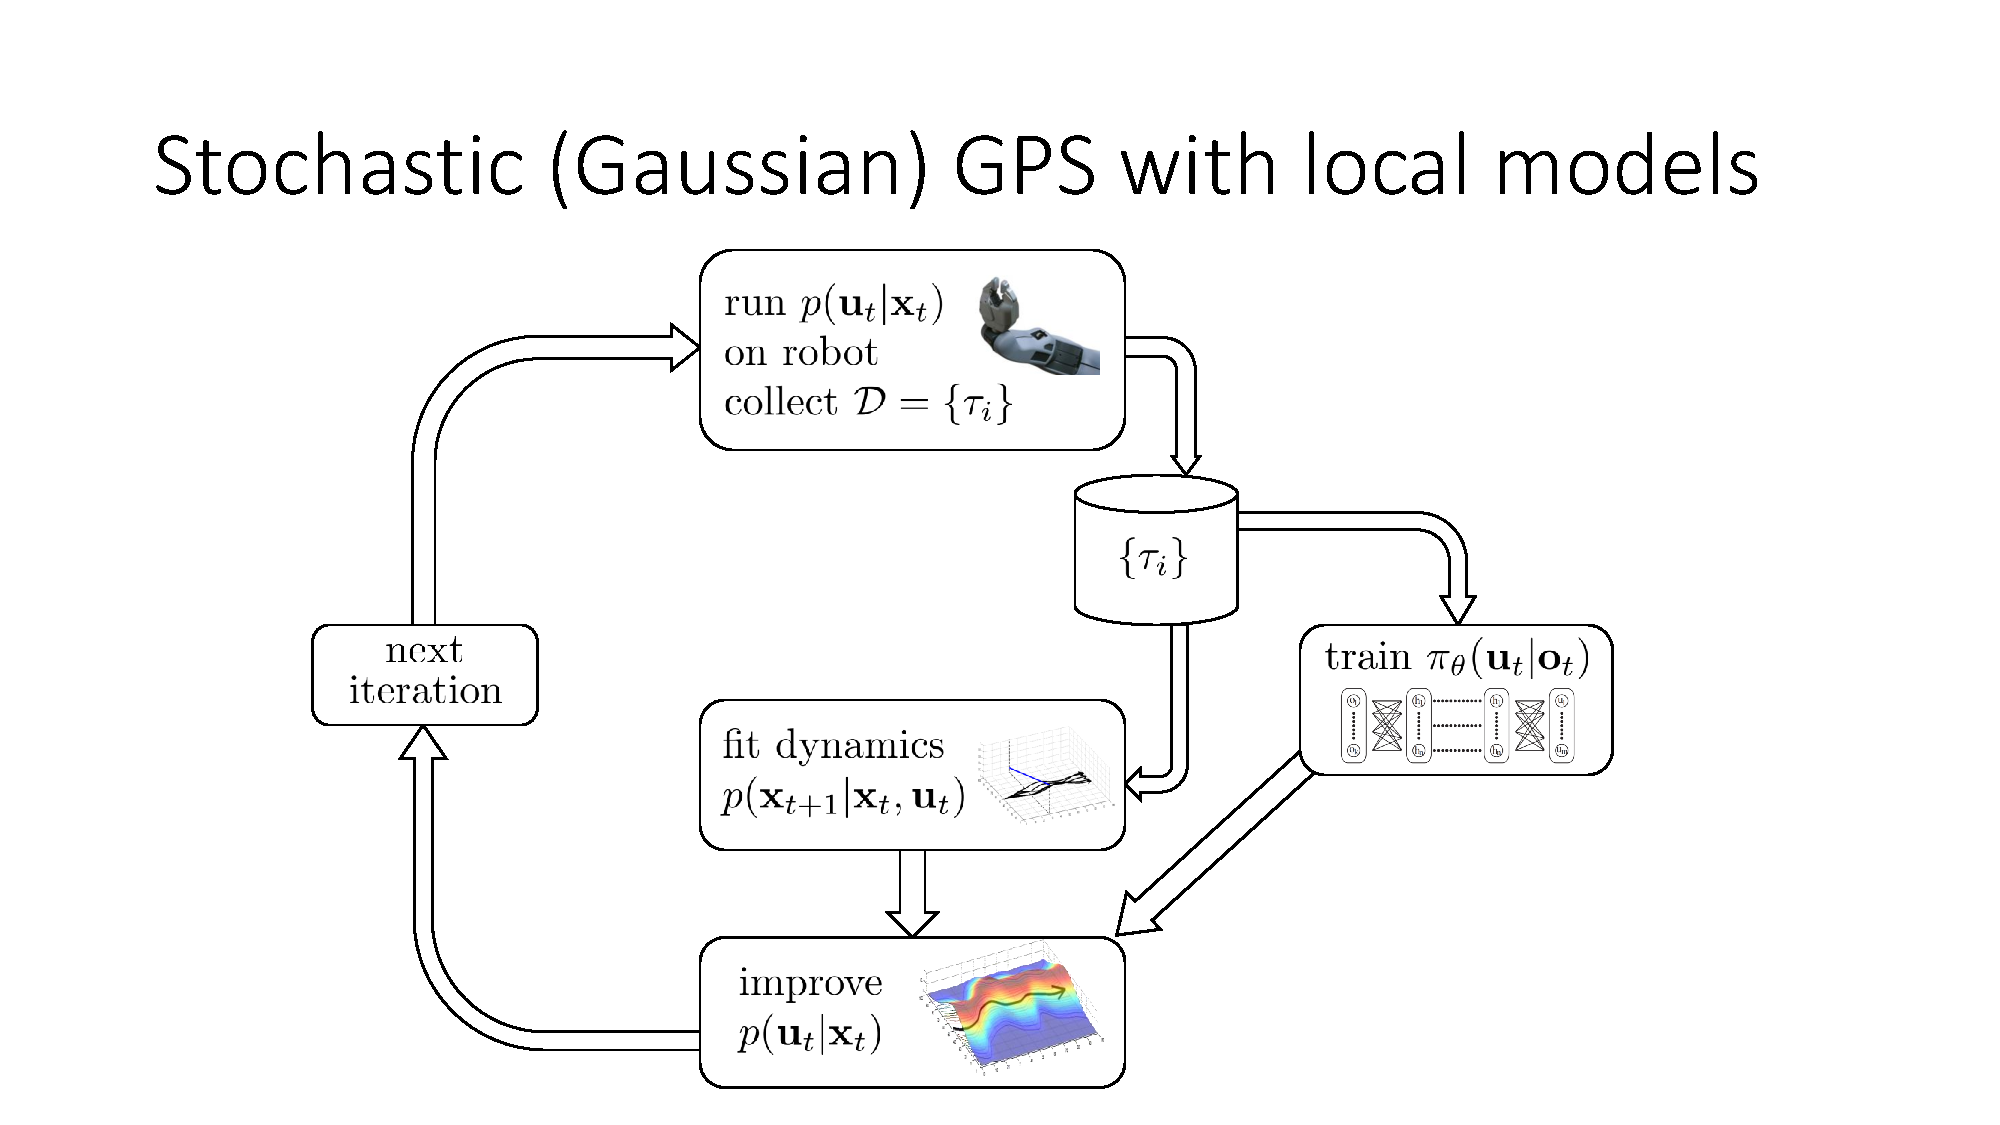
\includegraphics[width=0.8\linewidth]{img/GPS.png}
\end{figure}

\noindent\textbf{DAgger} 
\begin{figure}[H]
    \centering
        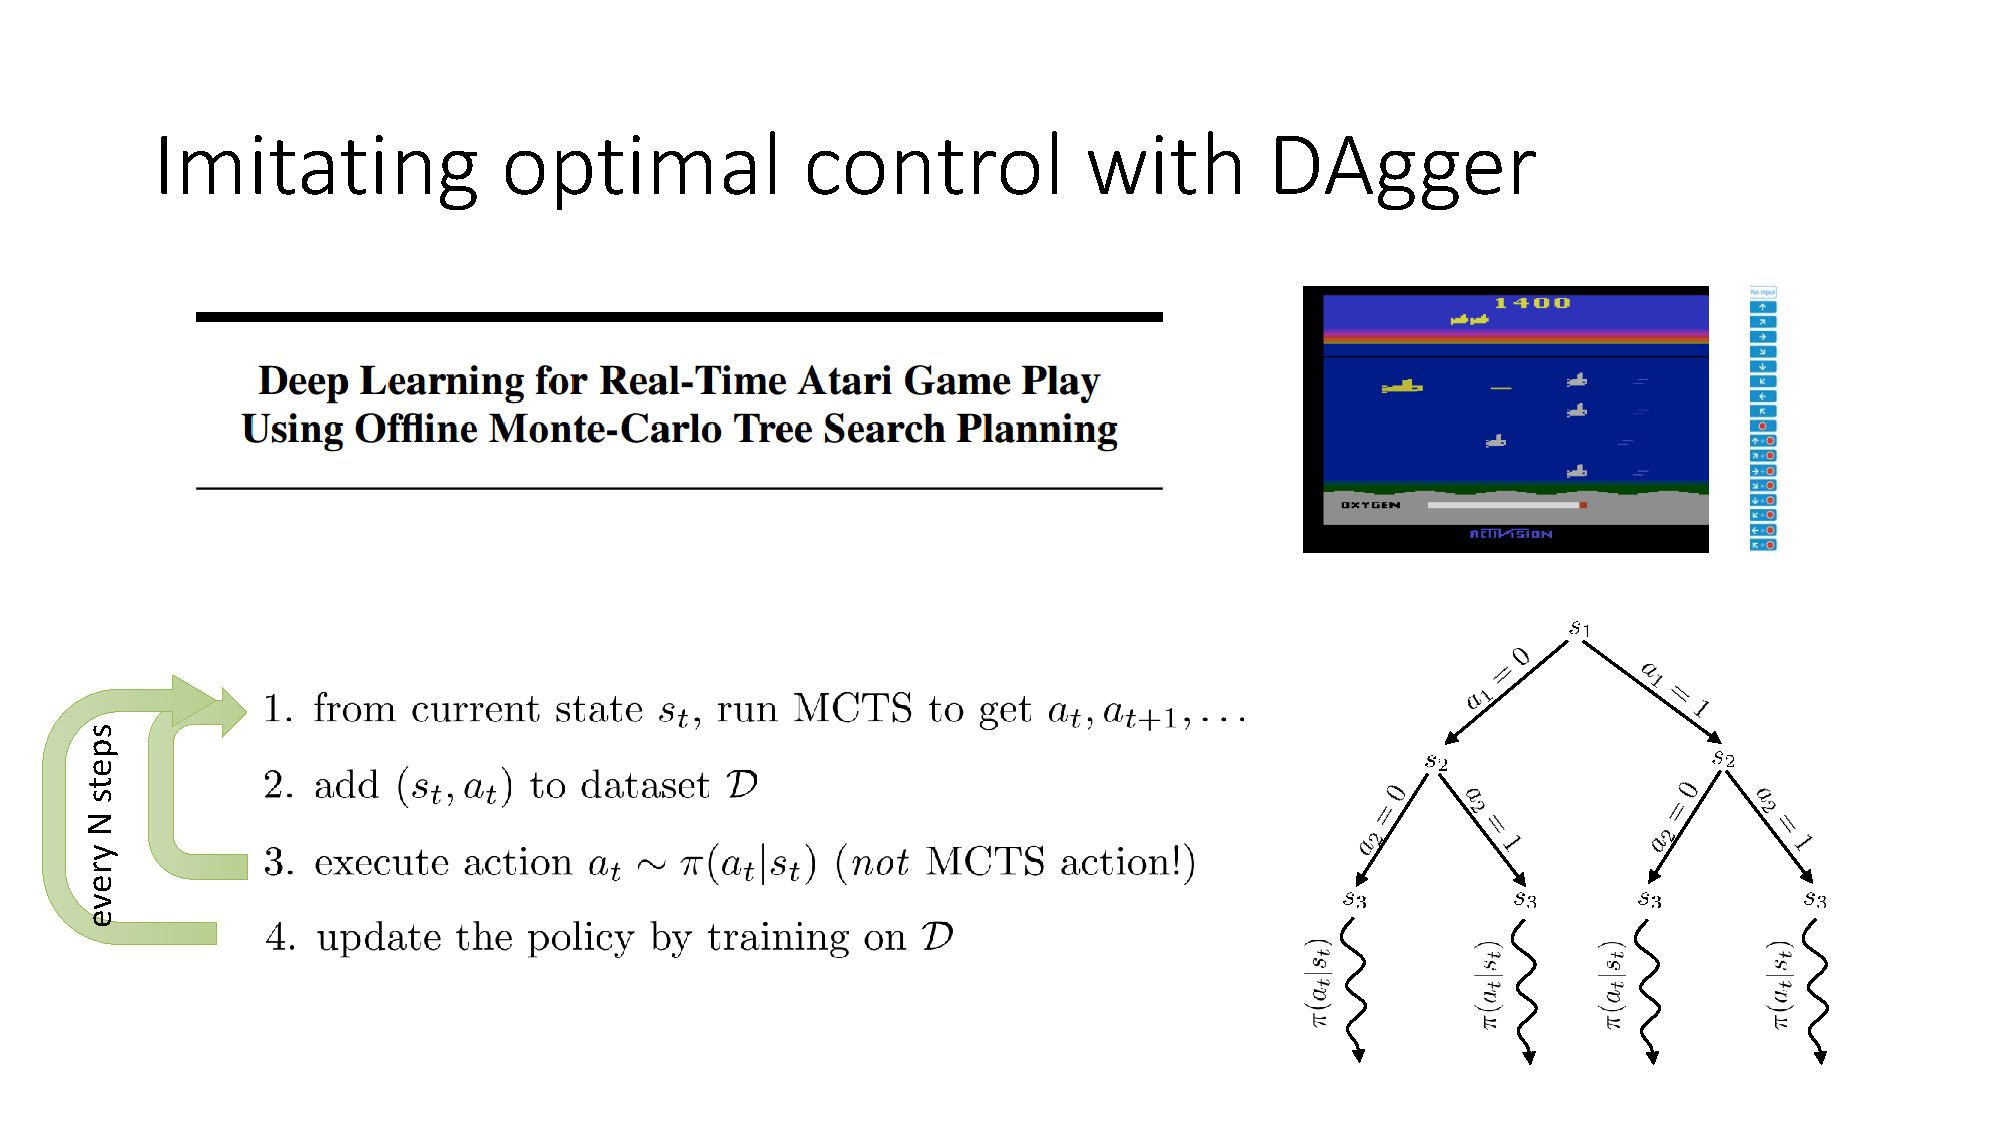
\includegraphics[width=0.8\linewidth]{img/DAgger.png}
\end{figure}

\noindent\textbf{PLATO} 

Dagger does not  care about how the actions are generated, it needs to make sure that actions are optimal with respect to the real reward function

\begin{figure}[H]
    \centering
        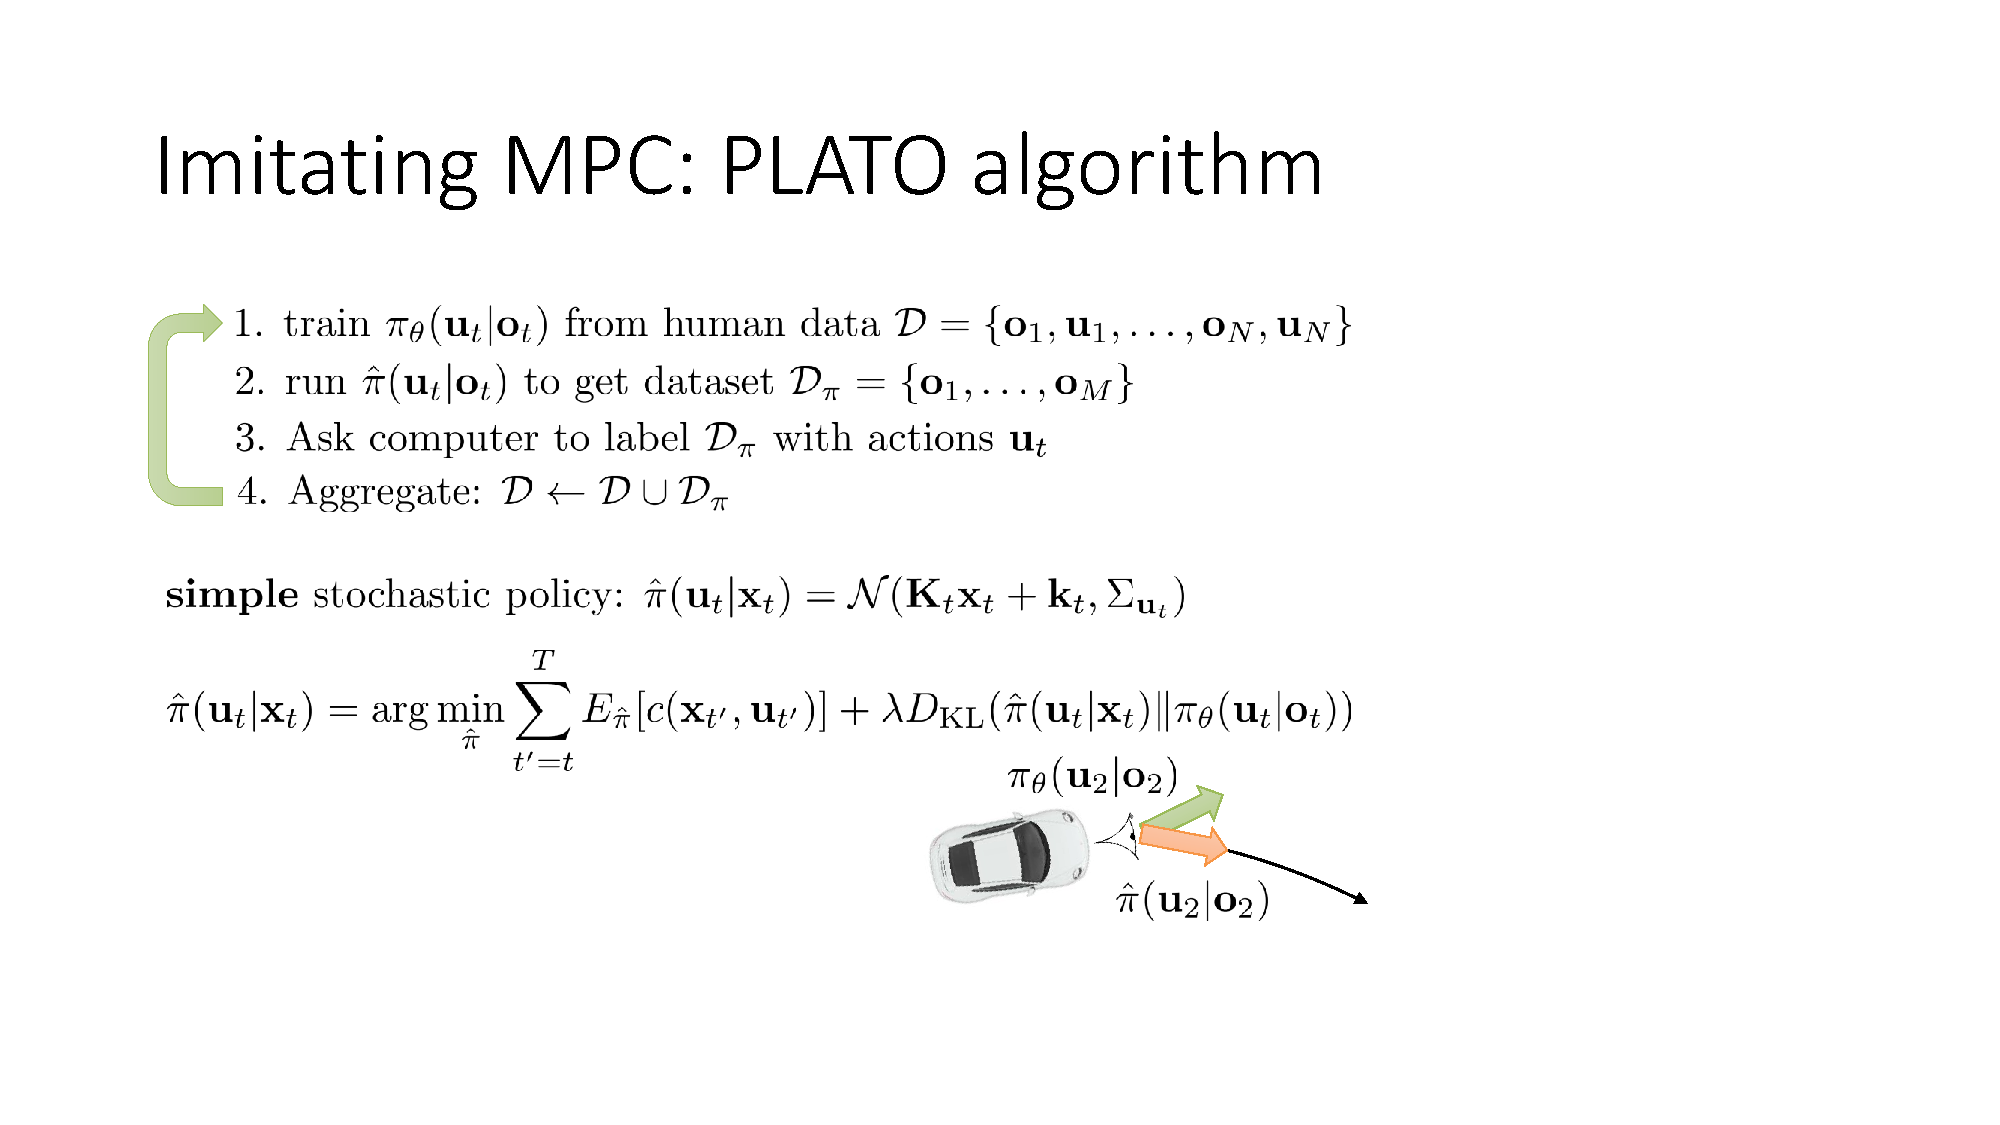
\includegraphics[width=0.8\linewidth]{img/PLATO.png}
\end{figure}

\noindent\textbf{DAgger vs GPS} 
\begin{figure}[H]
    \centering
        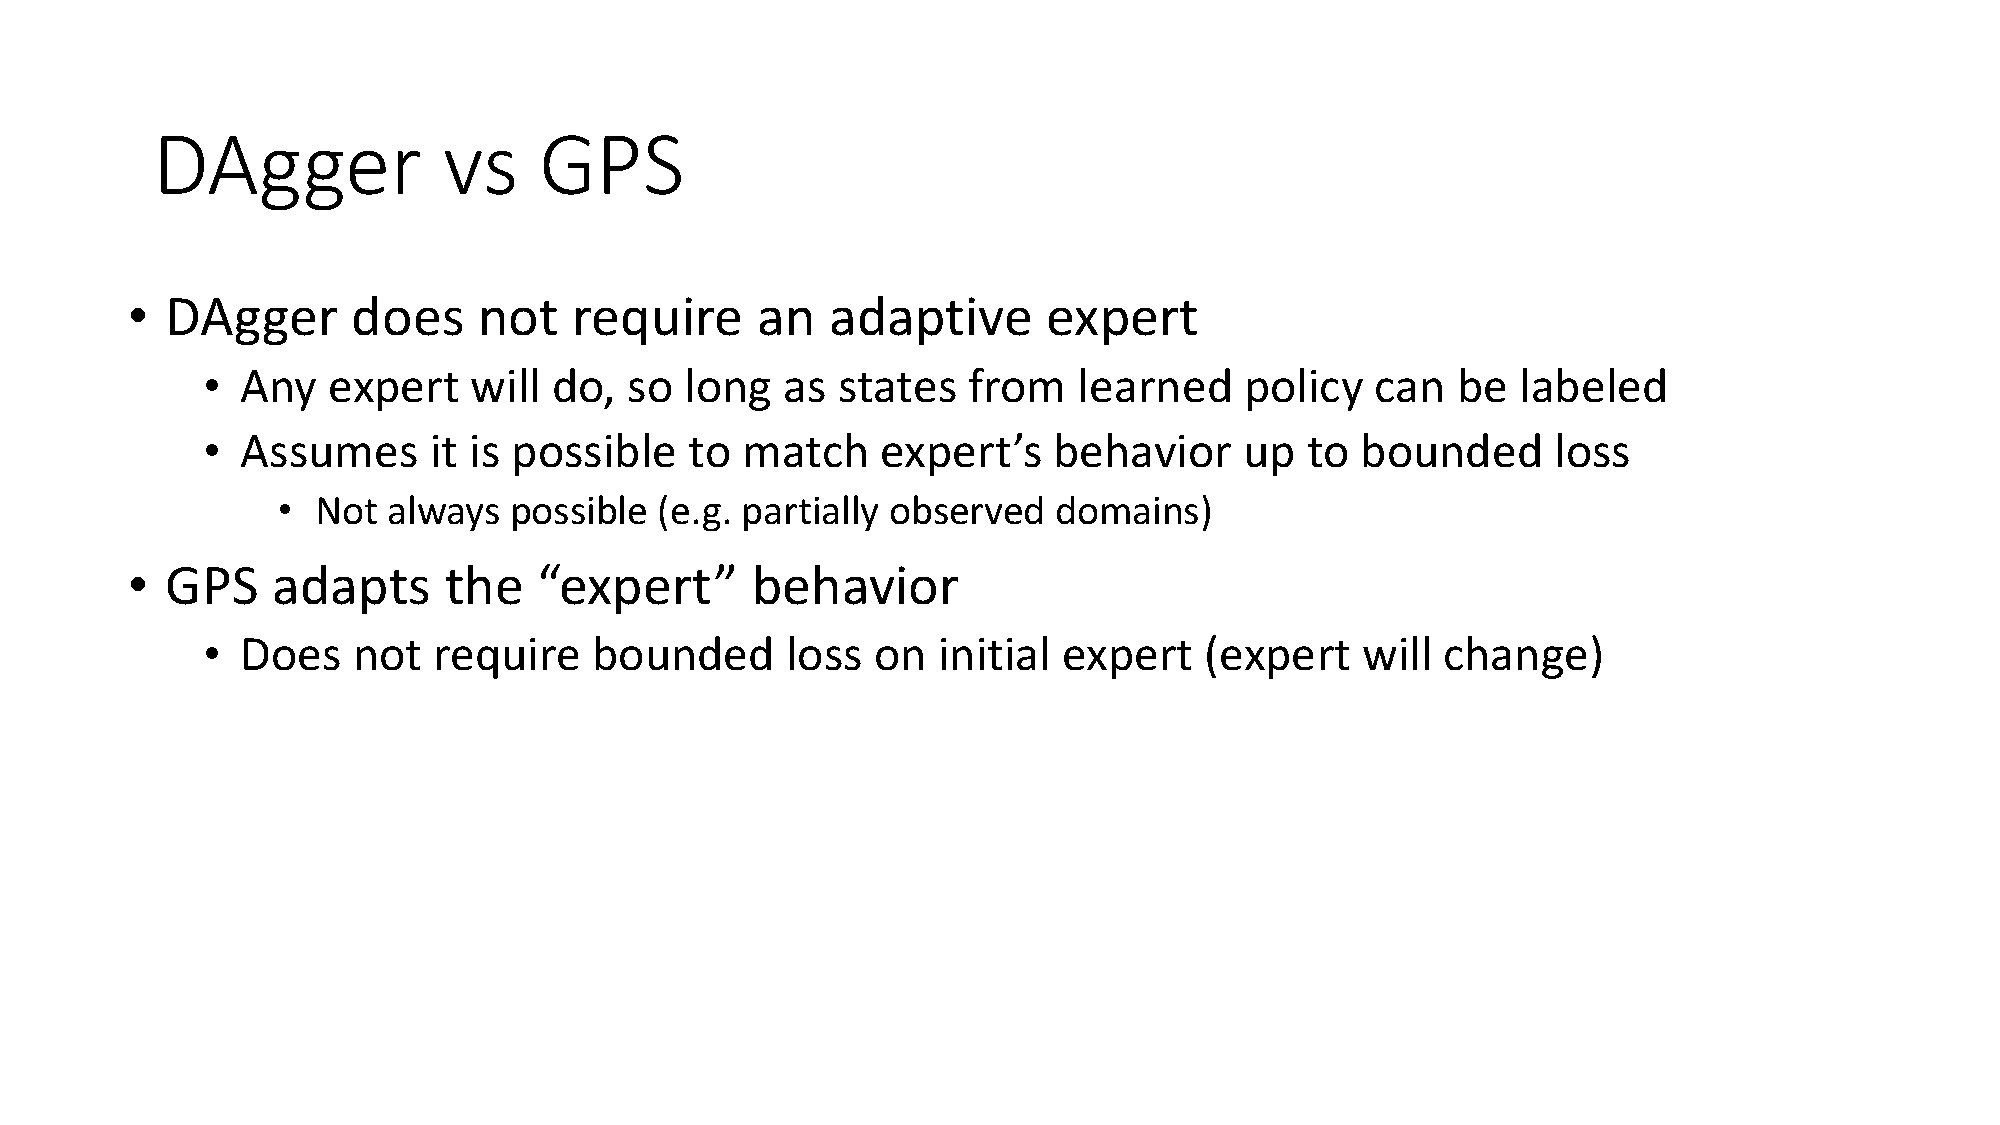
\includegraphics[width=0.8\linewidth]{img/DAgger_vs_GPS.png}
\end{figure}

\noindent\textbf{Why imitate?} 

\begin{itemize}
	\item It combines supervised learning and control and planning, which are stable and reliable to use
	\item Input is $o_t$ instead of $x_t$ for handling real observation
	\item get rid of numerical instability
\end{itemize}

\begin{figure}[H]
    \centering
        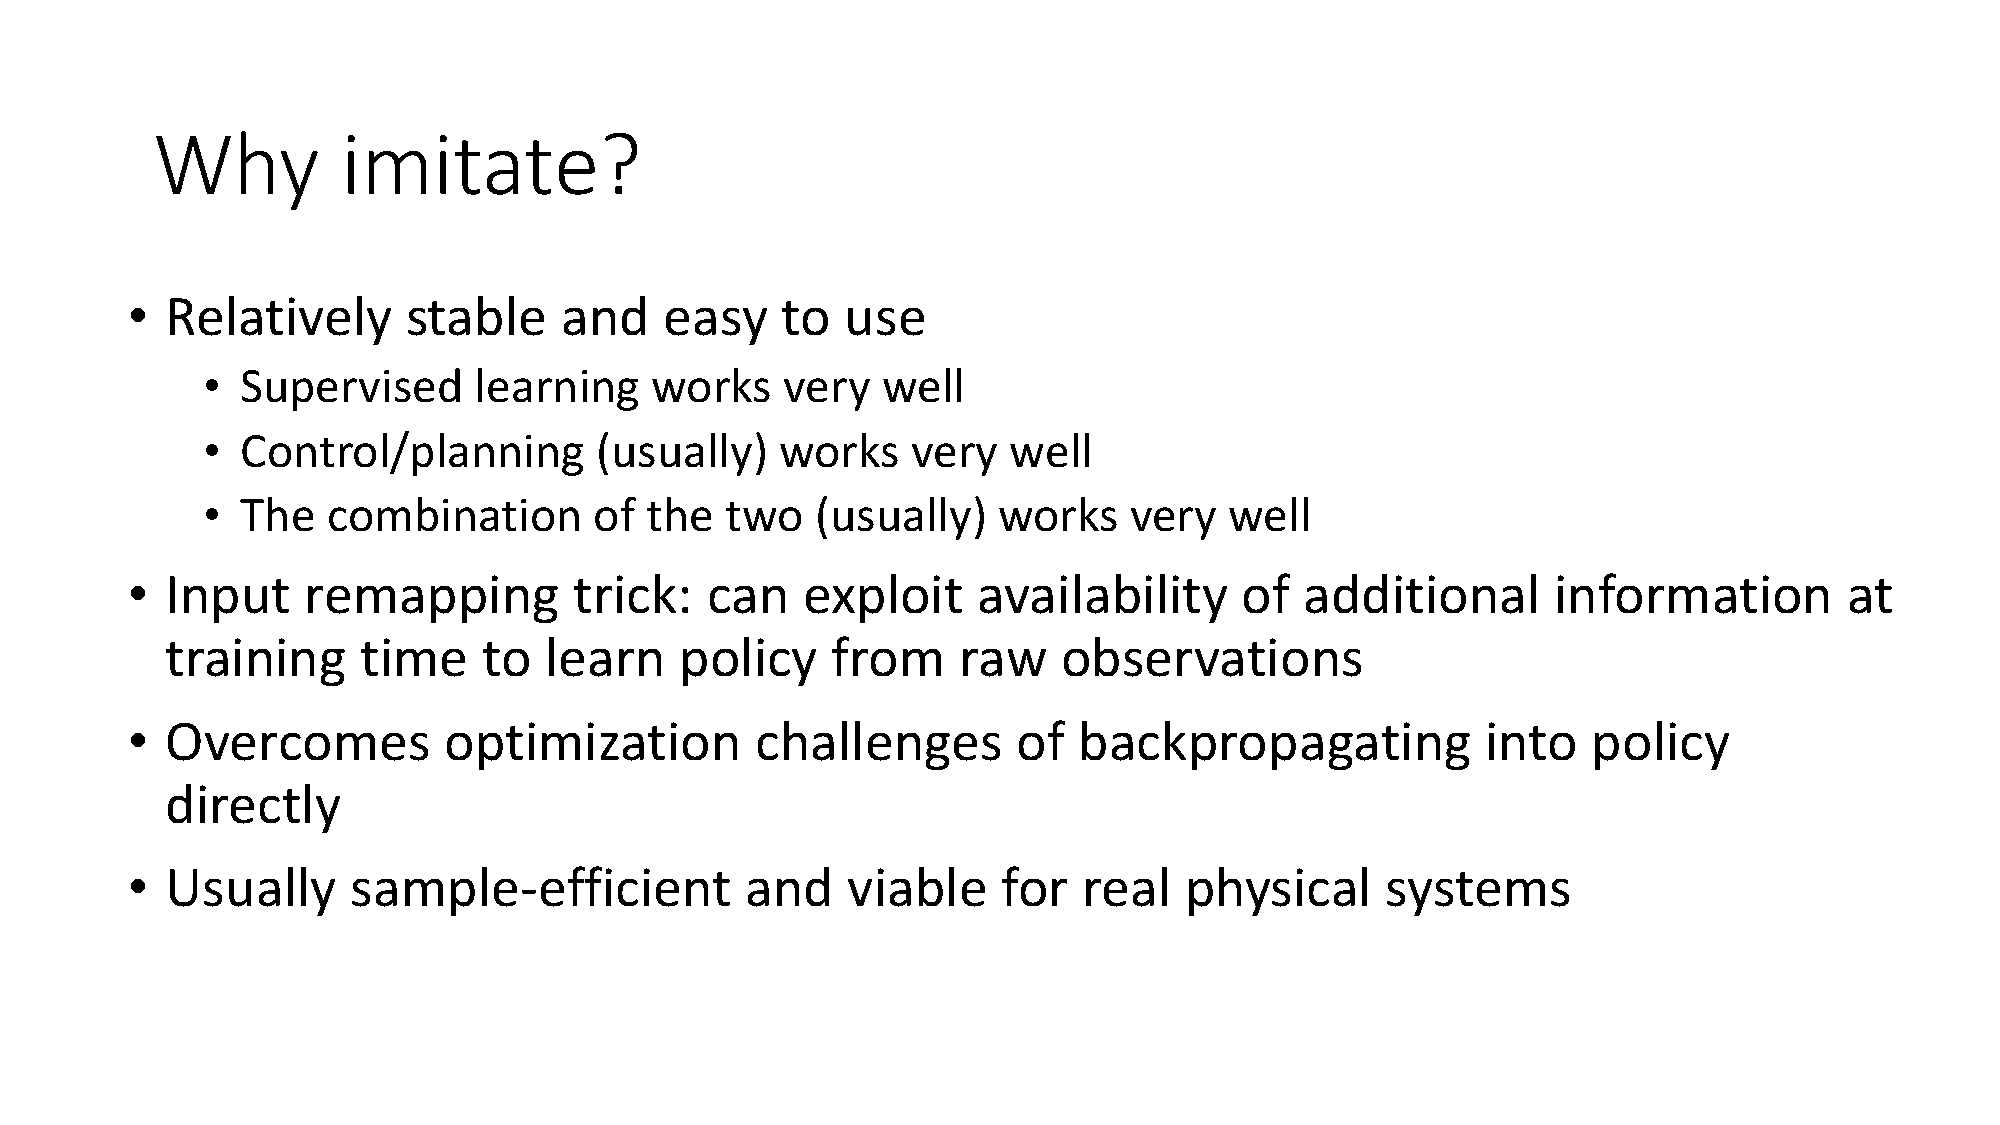
\includegraphics[width=0.8\linewidth]{img/why_imitate.png}
\end{figure}

\noindent\textbf{Dyna Algorithm} 

\begin{figure}[H]
    \centering
        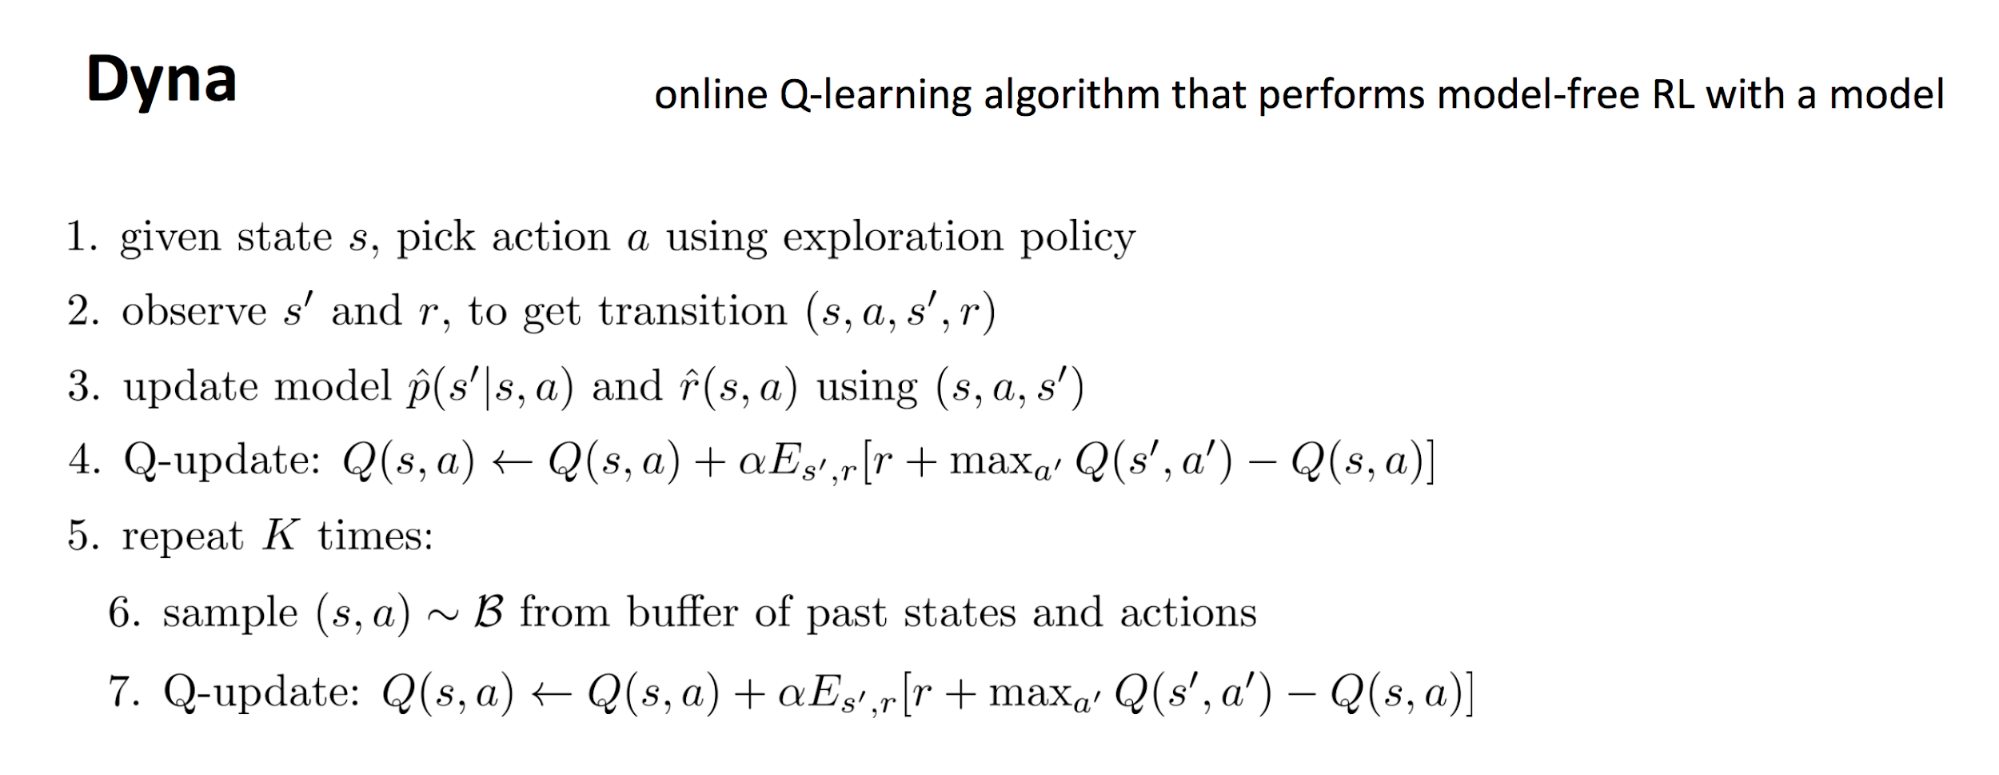
\includegraphics[width=0.8\linewidth]{img/Dyna.png}
\end{figure}

\begin{figure}[H]
    \centering
        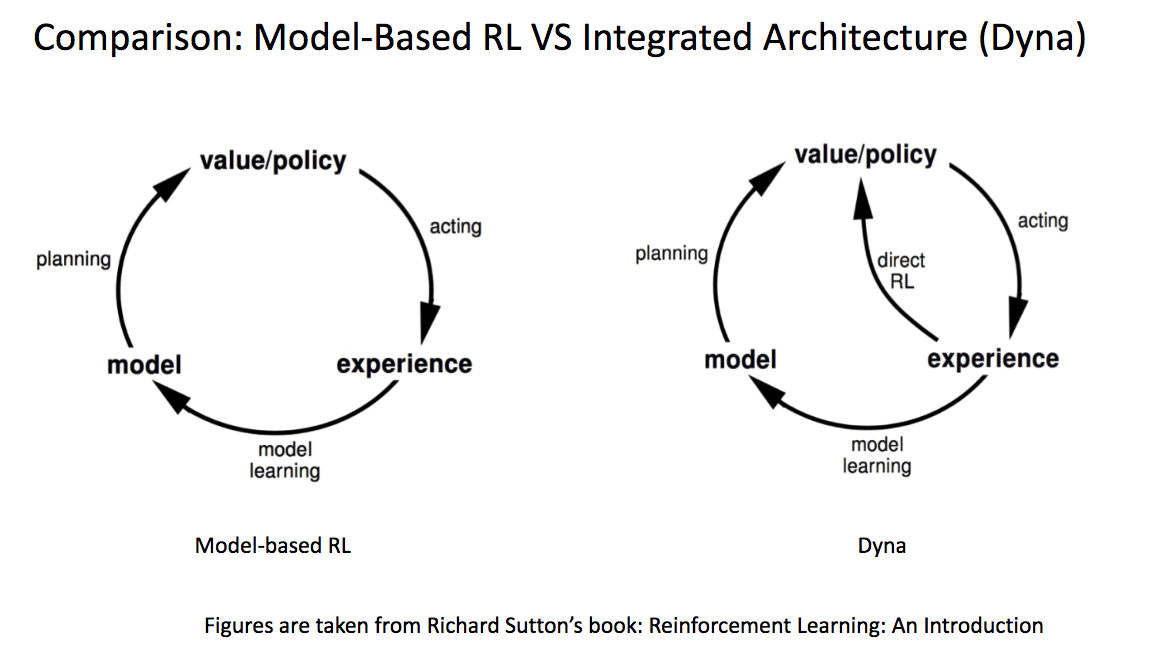
\includegraphics[width=0.8\linewidth]{img/Dyna_comparison.png}
\end{figure}

\begin{figure}[H]
    \centering
        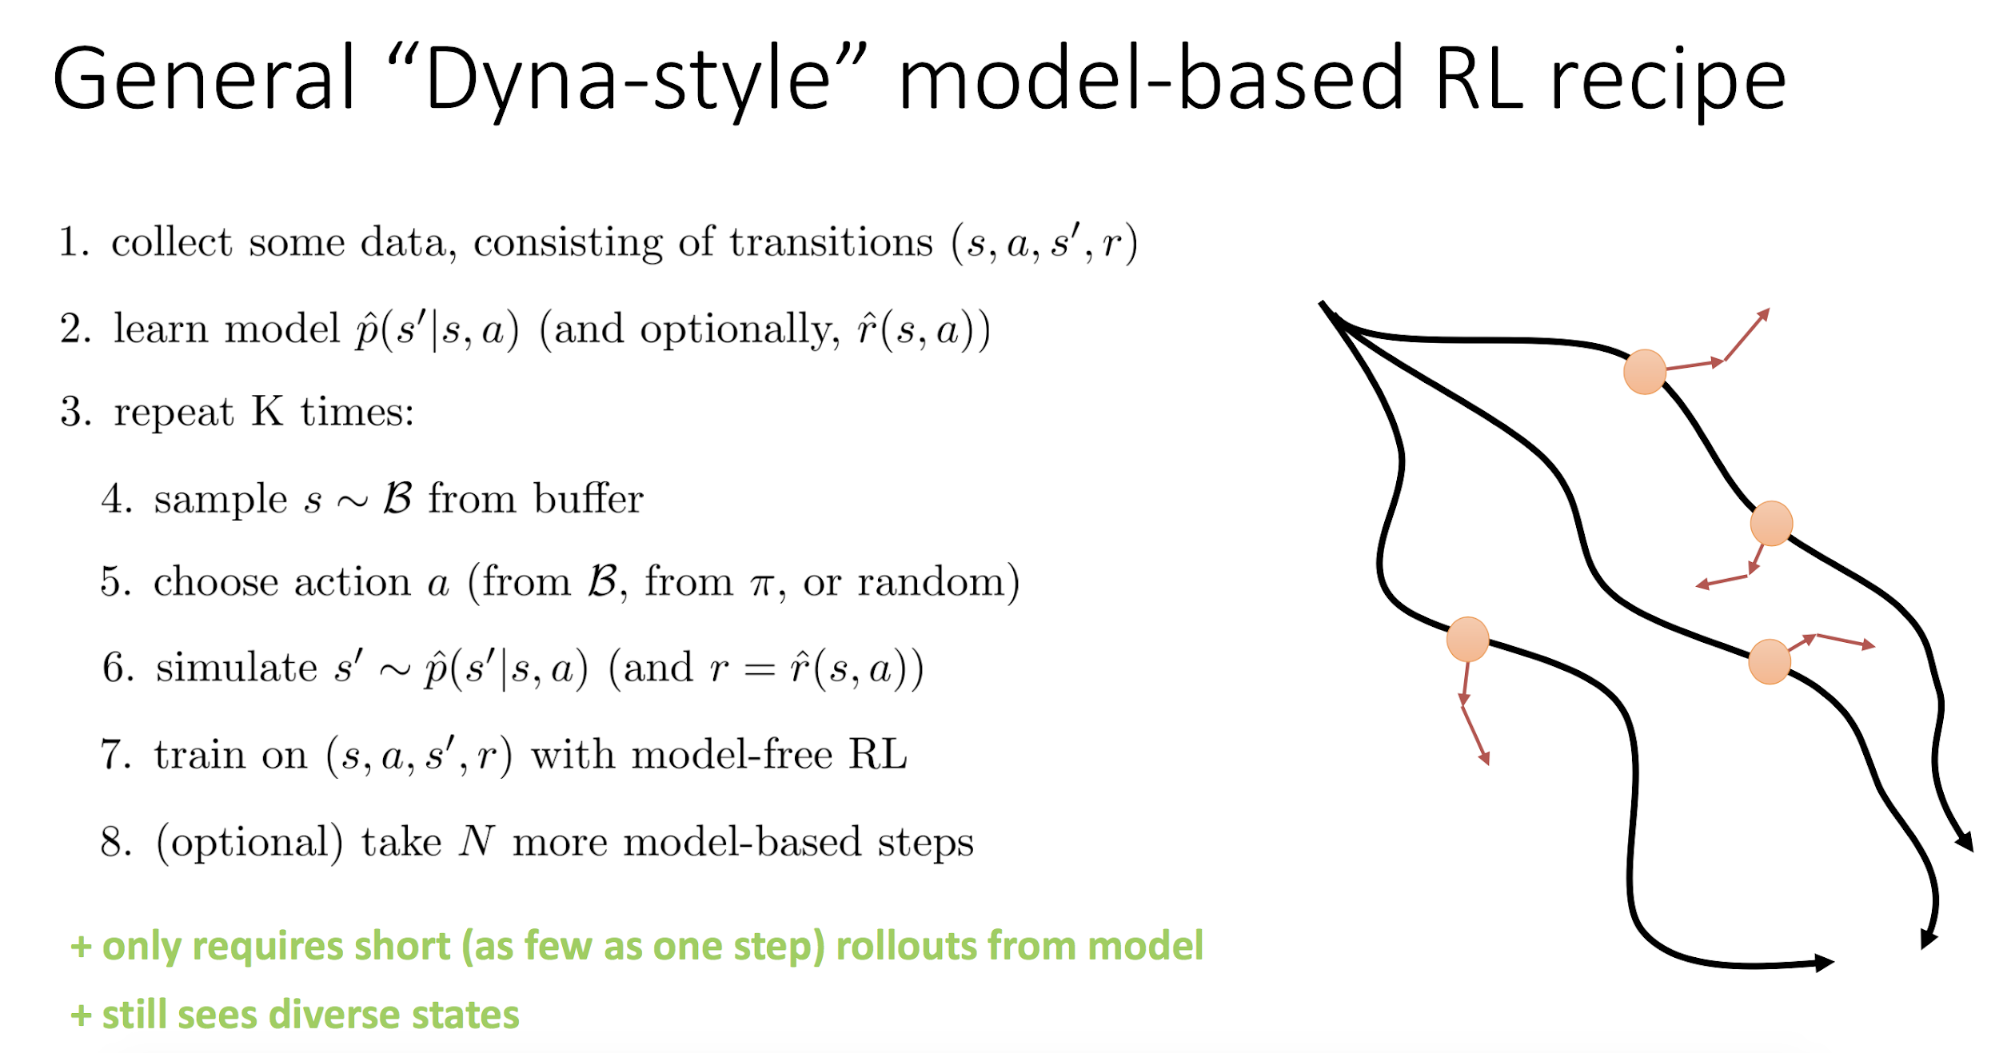
\includegraphics[width=0.8\linewidth]{img/general_Dyna.png}
\end{figure}

References
\begin{itemize}
	\item https://dl.acm.org/citation.cfm?id=122377
	\item https://medium.com/@ranko.mosic/online-planning-agent-dyna-q-algorithm-and-dyna-maze-example-sutton-and-barto-2016-7ad84a6dc52b
	\item https://www.cs.cmu.edu/afs/cs/project/jair/pub/volume4/kaelbling96a-html/node29.html
\end{itemize}

\section{Summary}
\begin{figure}[H]
    \centering
        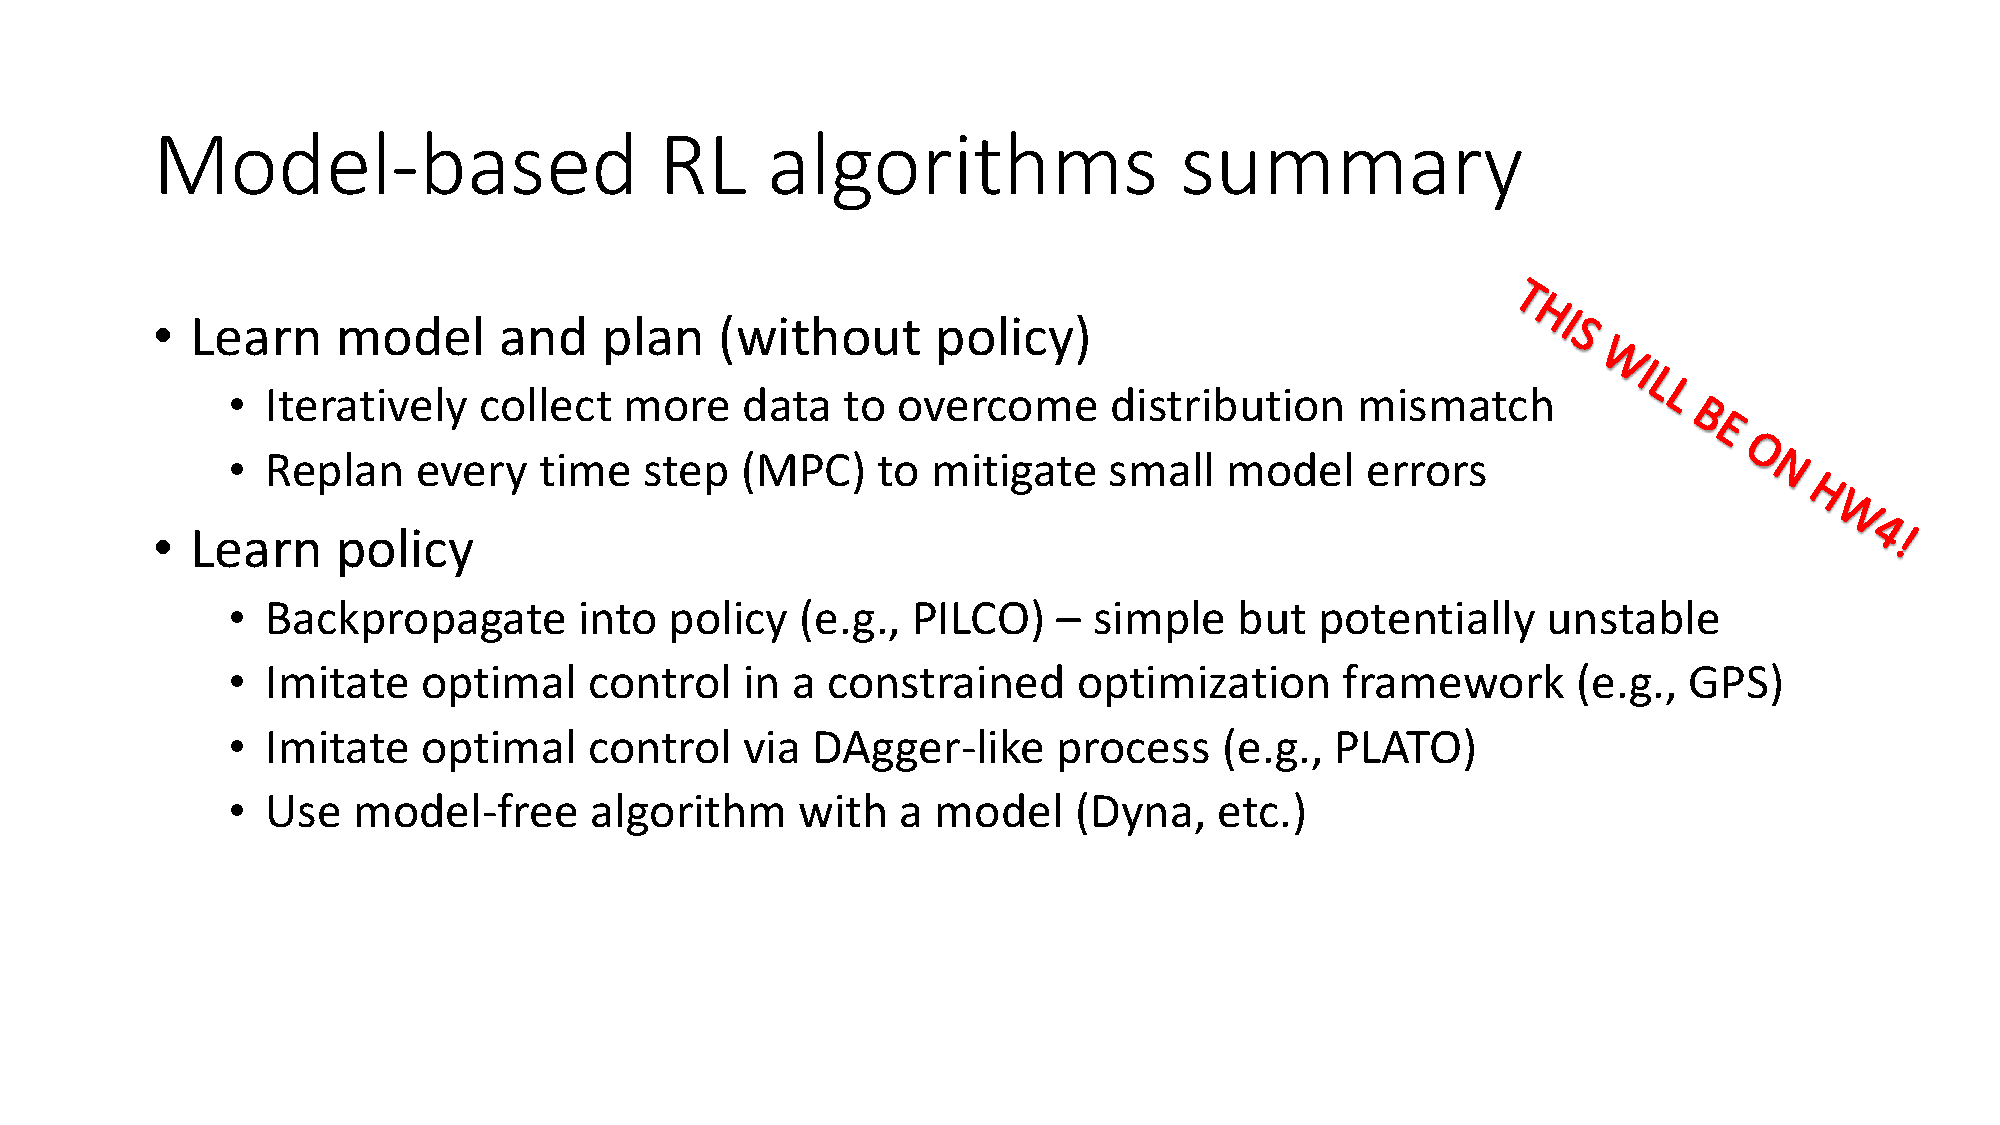
\includegraphics[width=0.8\linewidth]{img/model-based.png}
\end{figure}

\begin{figure}[H]
    \centering
        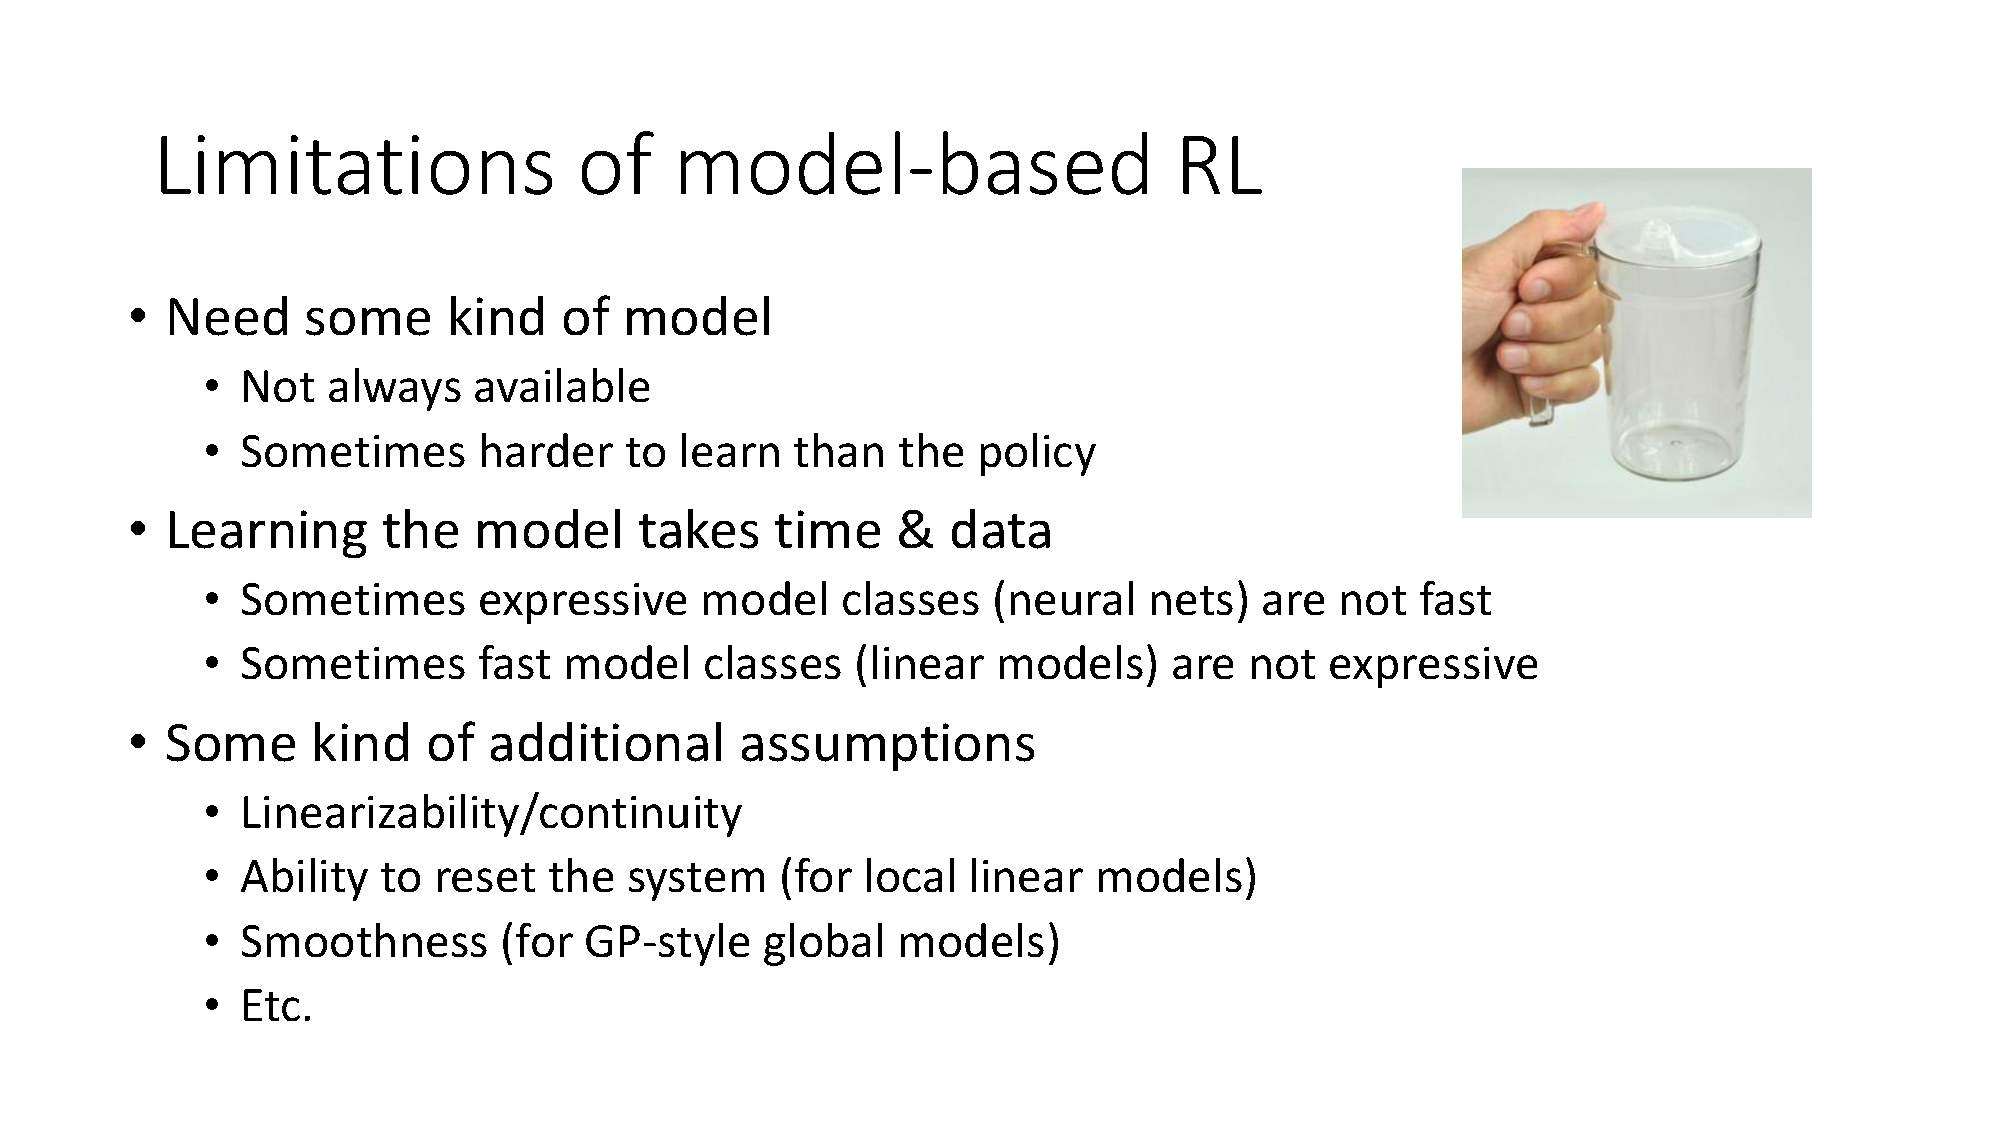
\includegraphics[width=0.8\linewidth]{img/model-based-limitations.png}
\end{figure}

\begin{figure}[H]
    \centering
        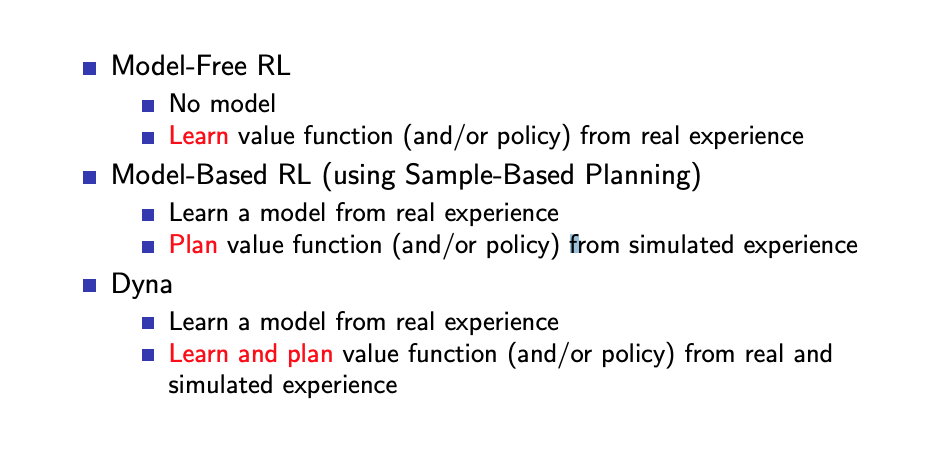
\includegraphics[width=0.8\linewidth]{img/summary.png}
\end{figure}

\section{Questions}

1. Why quadratic loss in the second term
\begin{figure}[H]
    \centering
        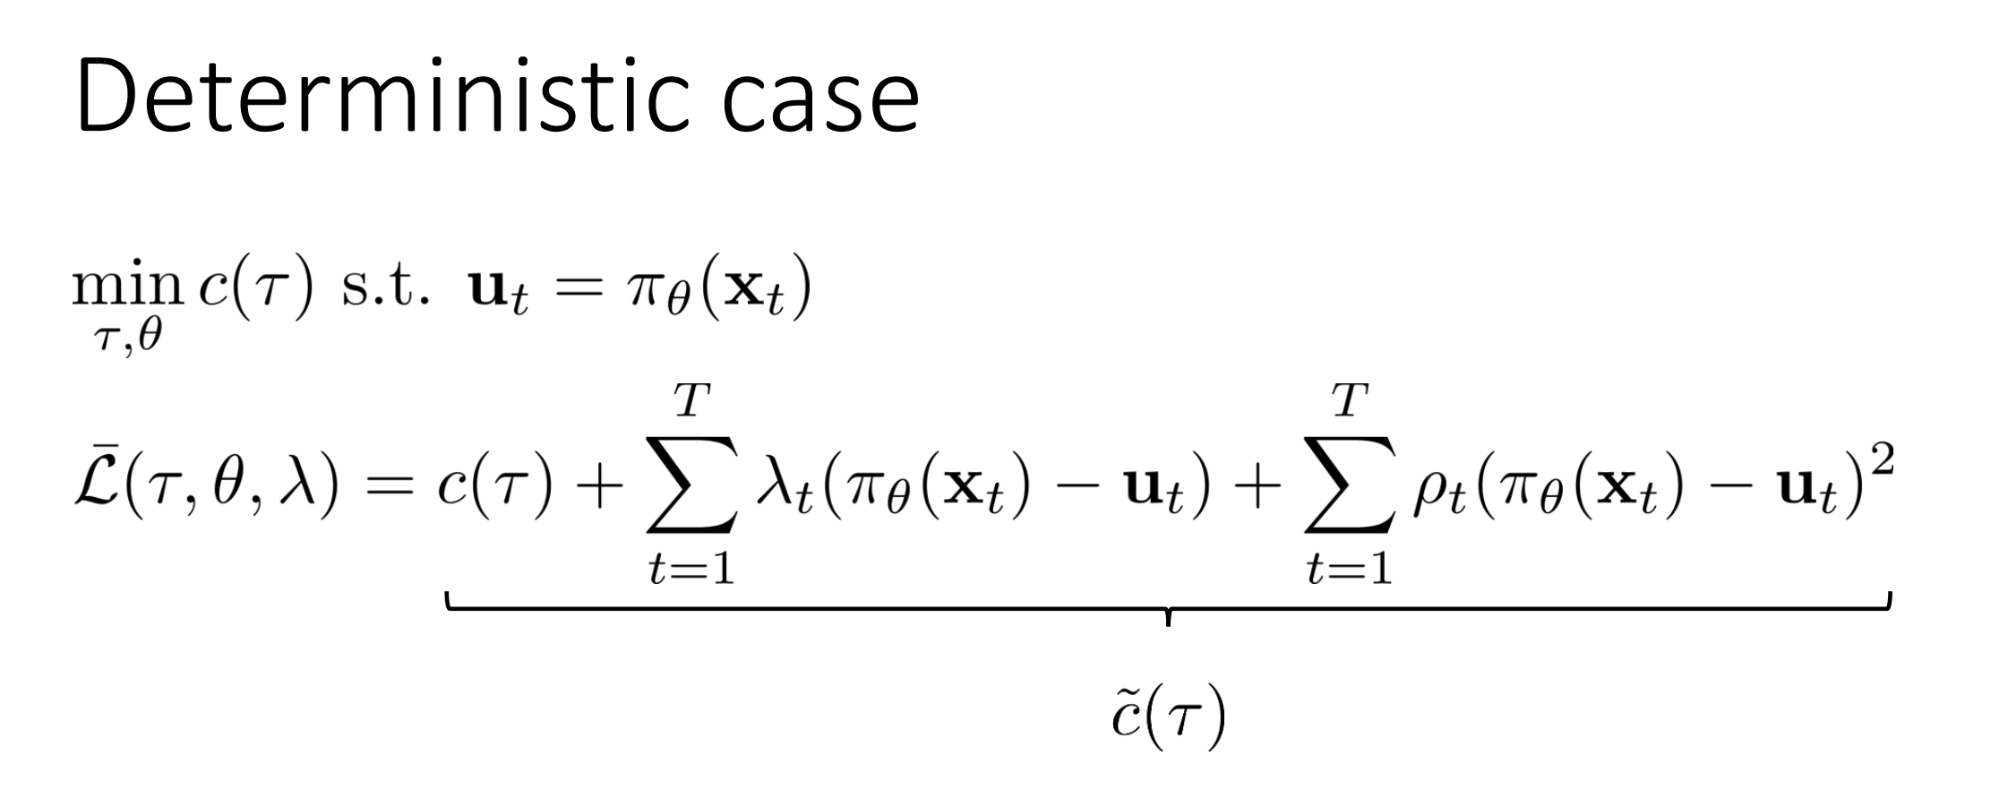
\includegraphics[width=0.8\linewidth]{img/deterministic.png}
\end{figure}

2. Is iLQR a shooting method or a collocation method

https://people.eecs.berkeley.edu/~pabbeel/cs287-fa11/slides/NonlinearOptimizationForOptimalControl-part2.pdf

% References
\small
\bibliographystyle{plain}
\bibliography{bibliography}
\end{document}
